\begin{slide}{Visualization Tools}
  \begin{itemize}
    \item<2-> Deep Neural Networks have the tendency of being \dots\, deep
    \item<3-> Easy to drown in the complexity of an architecture
    \item<4-> $>$ 36,000 nodes for Google's \emph{Inception} model
  \end{itemize}
  \onslide<5->{
    \begin{figure}
      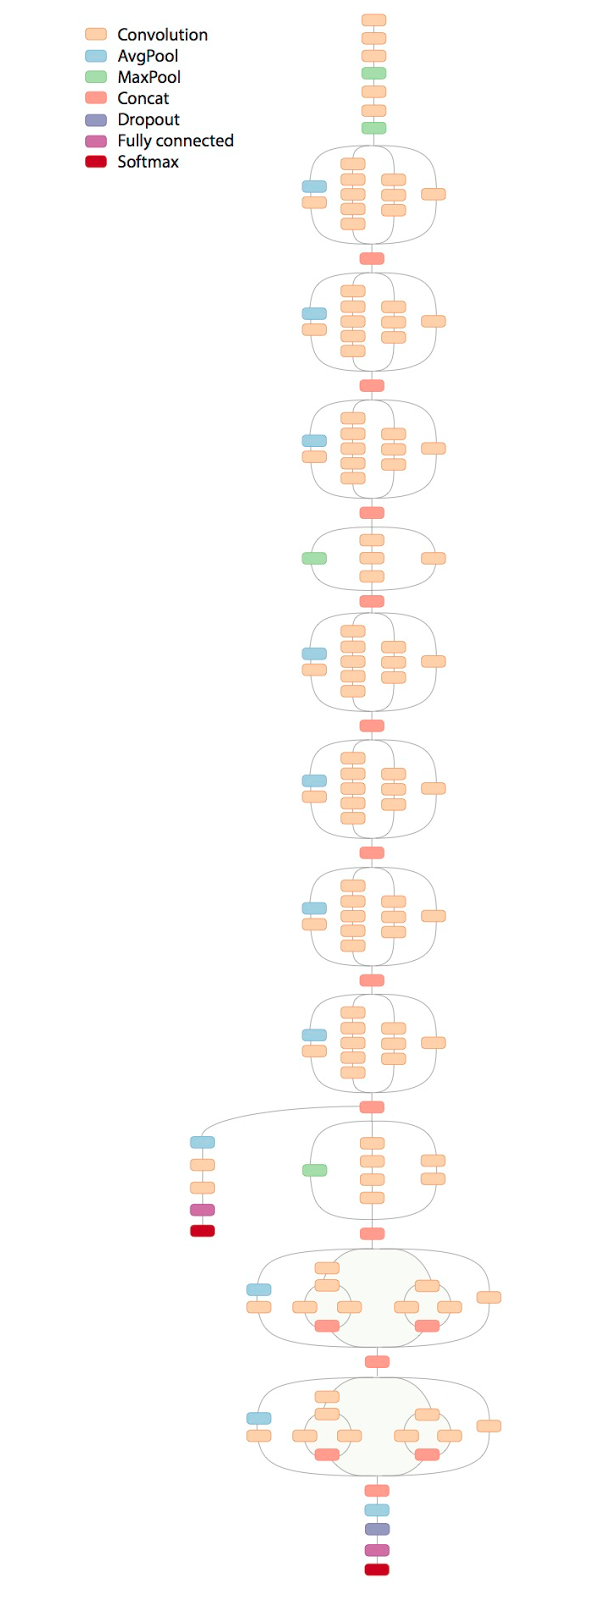
\includegraphics[scale=0.5, trim={0 50cm 0 0}, clip]{inception}
    \end{figure}
  }
\end{slide}

\begin{frame}
  \begin{figure}
     \advance\leftskip-2.2cm
    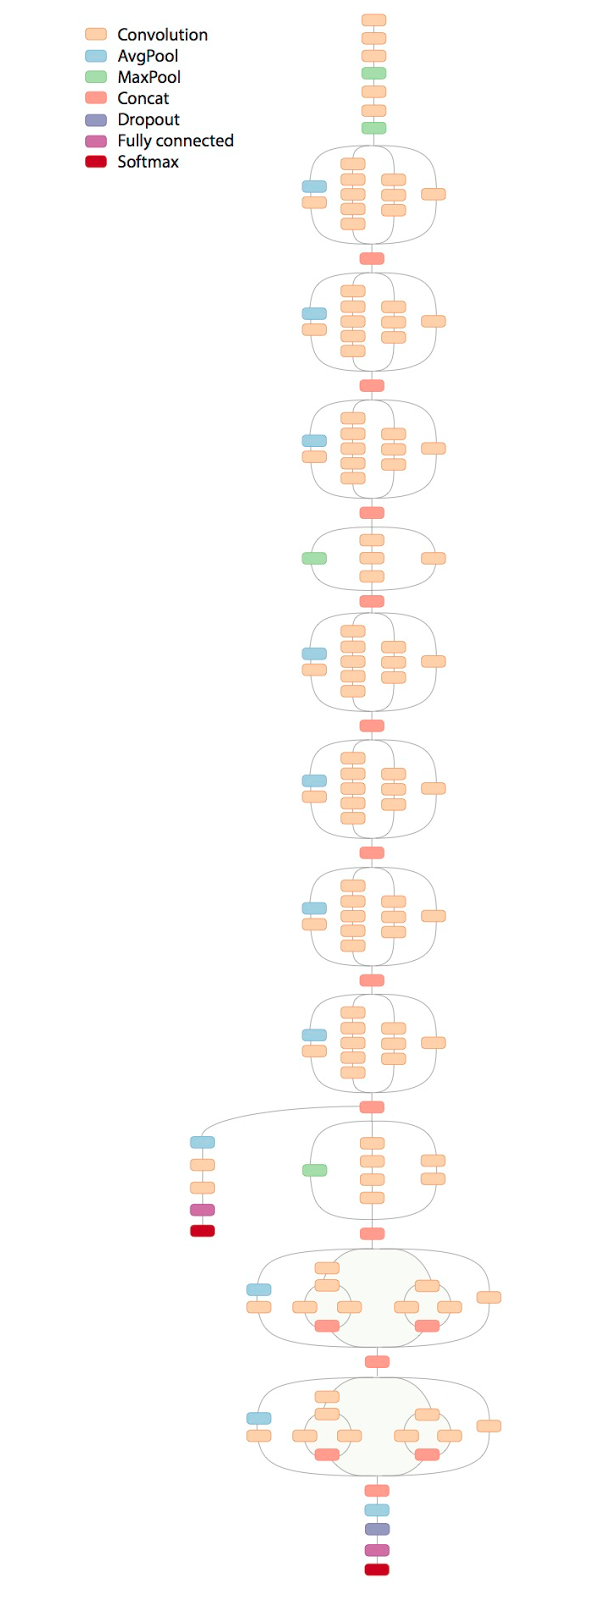
\includegraphics[scale=0.5, trim={0 32cm 0 11cm}, clip]{inception}
  \end{figure}
\end{frame}

\begin{frame}
  \begin{figure}
    \advance\leftskip-2.2cm
    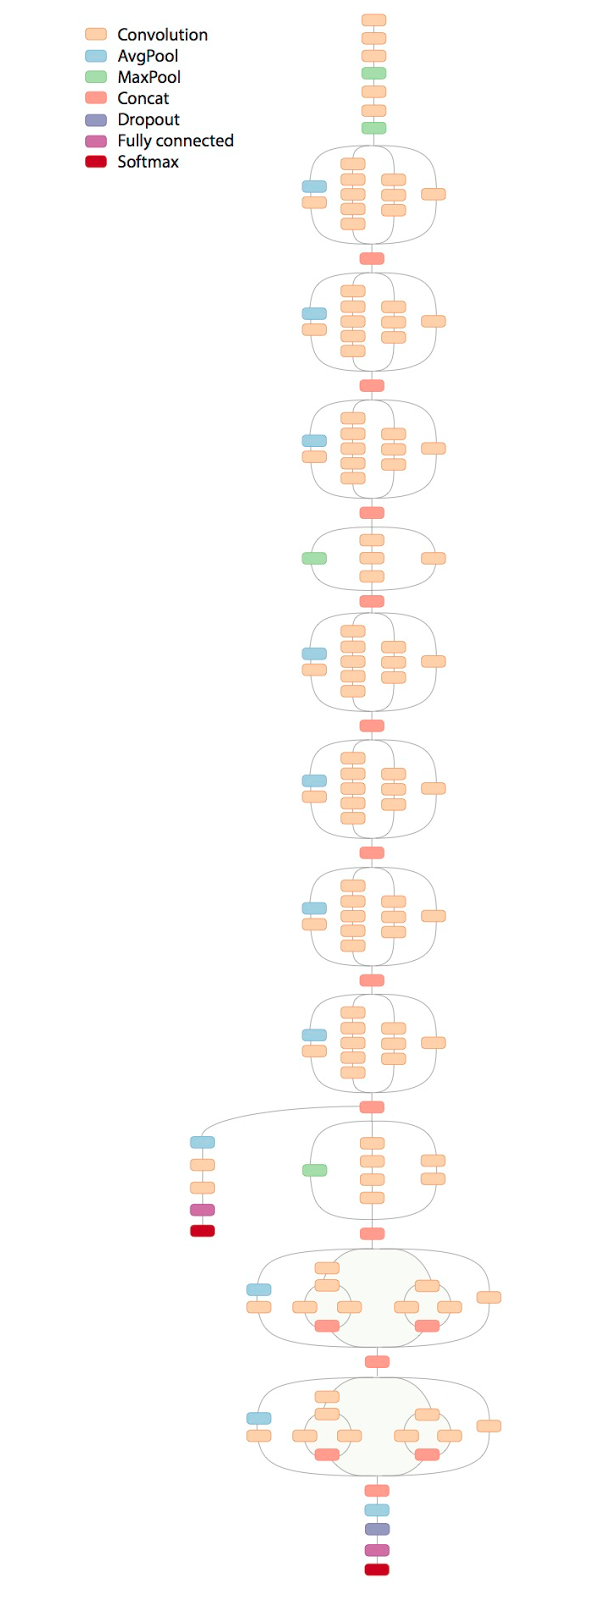
\includegraphics[scale=0.5, trim={0 20cm 0 23.7cm}, clip]{inception}
  \end{figure}
\end{frame}

\begin{frame}
  \begin{figure}
    \advance\leftskip-2.2cm
    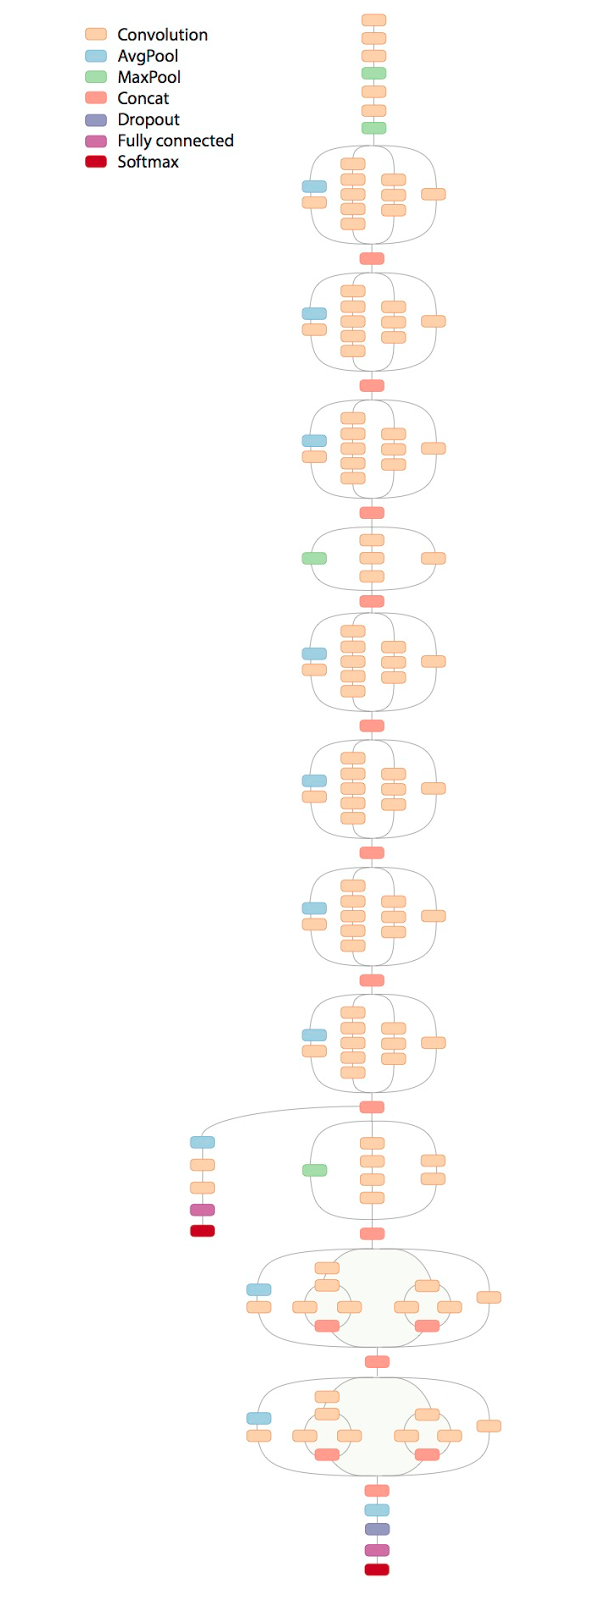
\includegraphics[scale=0.5, trim={0 5cm 0 36.5cm}, clip]{inception}
  \end{figure}
\end{frame}

\begin{frame}
  \begin{figure}
    \advance\leftskip-2.2cm
    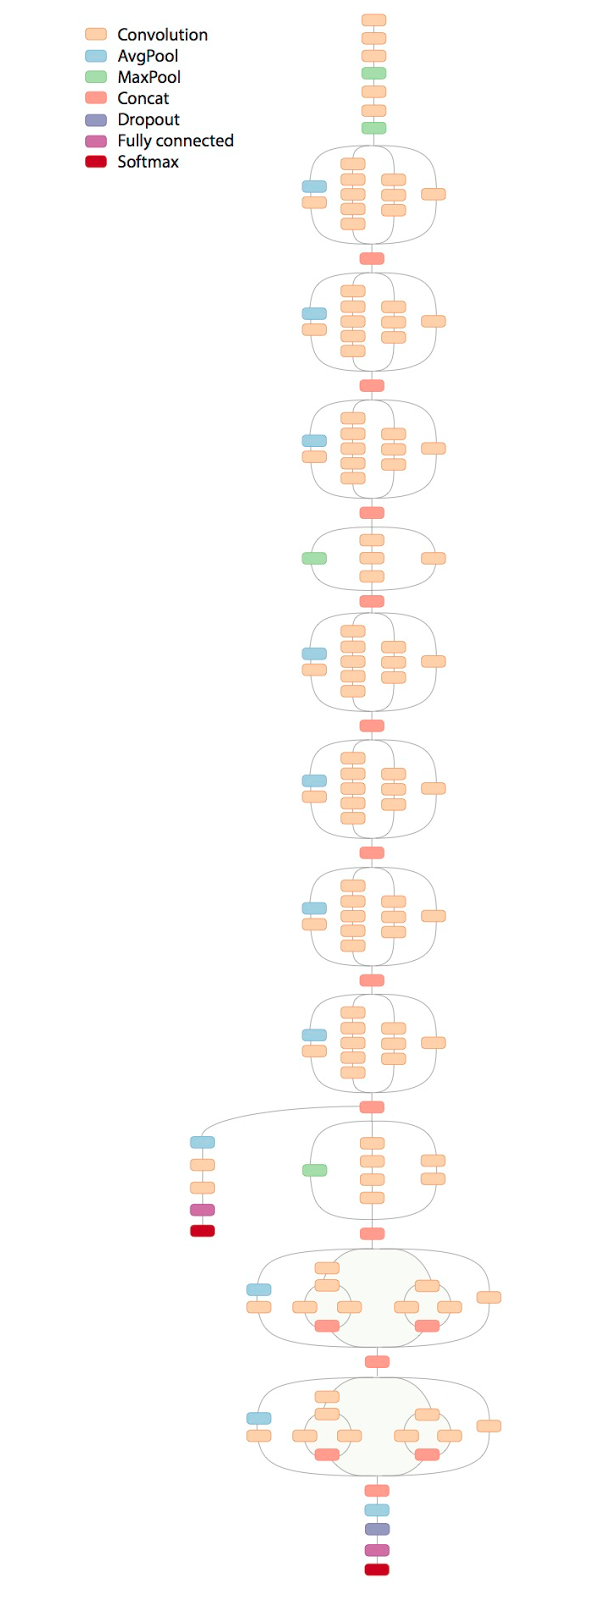
\includegraphics[scale=0.5, trim={0 0 0 51.3cm}, clip]{inception}

    \onslide<2->{
    \hspace{3cm}
\includegraphics[scale=0.15]{gold}
    \vfill
    }
  \end{figure}
  {\tiny Source: http://googleresearch.blogspot.de/2016/03/train-your-own-image-classifier-with.html}
\end{frame}

\textframe{\href{http://0.0.0.0:6006}{TensorBoard to the Rescue}}

%%% Local Variables:
%%% mode: latex
%%% TeX-master: "../presentation"
%%% End:
